\part{Polarisation circulaire, molécules chirales et harmoniques d'ordre élevé}
\label{PA:Spin_HHG}
\chapter{Génération d'harmoniques d'ordre élevé polarisée elliptiquement}
\label{CH:Circular_HHG}
Dans cette partie nous présenterons comment générer des harmoniques d'ordre élevé portant du moment angulaire de spin, c'est-à-dire ayant une polarisation elliptique. Nous présenterons pour commencer le formalisme utile à la description d'ondes polarisées, puis étudierons le mécanisme de GHOE dans un atome quand le laser de génération est polarisé elliptiquement. Nous verrons que ce mécanisme présente des difficultés intrinsèques et mentionnerons les solutions existantes, avant d'en démontrer une nouvelle qui utilise une résonance de l'atome ou la molécule de génération.

\section{Formalisme pour la description d'ondes polarisées elliptiquement}
\label{sec:polardef}
Comme on l'a vu dans la partie \ref{sec:circpolar}, le champ électrique d'une onde polarisée elliptiquement décrit une ellipse au cours de sa propagation. Soit $(x,y,z)$ un repère cartésien tel que $z$ soit selon la direction de propagation et $x$ selon l'axe majeur de l'ellipse. Le champ, que l'on considère monochromatique, s'écrit :
\begin{equation}
\bm{E}=\begin{pmatrix}
E_{x}\cos{(\omega t-kz)}\\
E_{y}\sin{(\omega t-kz)}\\
0
\end{pmatrix}=E_{0}
\begin{pmatrix}
\cos{(\omega t-kz)}\\
\epsilon\sin{(\omega t-kz)}\\
0
\end{pmatrix},
\label{eq:jones}
\end{equation}
où $\epsilon = E_{y}/E_{x}$ est appelé ellipticité du champ. $\epsilon$ varie de 0 pour une polarisation linéaire à 1 pour une polarisation circulaire.  On a vu que si $\epsilon>0$ (resp. $<0$), l'onde était elliptique gauche (resp. droite) et porte un moment angulaire de spin de $\hbar$ (resp. $-\hbar$). 

\begin{figure}[!ht]
\centering
\def\svgwidth{0.6\columnwidth}
\import{Figures/Polar/}{polarellipse.pdf_tex}
\caption{Définition des différents paramètres de l'ellipse de polarisation.}
\label{Fig:polarellipse}
\end{figure}
Dans un repère où $x$ et $y$ ne sont pas selon les axes de l'ellipse (voir figure \ref{Fig:polarellipse}), on note $\eta$ l'angle entre l'axe $x$ et l'axe majeur de l'ellipse. L'ellipticité est déterminée par le rapport des axes mineurs et majeurs de l'ellipse, $b$ et $a$ : $\epsilon = b/a$. On note $\chi$ l'angle tel que $\tan\chi = \epsilon = b/a$. Comme les amplitudes du champ selon les axes de l'ellipse sont déphasées de $\pi/2$, $a$ et $b$ peuvent être vus comme les parties réelle et imaginaire d'un vecteur de polarisation complexe et unitaire $\bm{\Pi}$. Le champ s'écrit alors :
\[\bm{E} = E_x \bm{e_x} + E_y \bm{e_y} = E_0(\Pi_x \bm{e_x} + \Pi_y \bm{e_y}).\] 
Il sera utile d'utiliser les \textit{paramètres de Stokes}, définis comme :
\begin{align}
S_0 &= E_xE_x^*+E_yE_y^* =E_0^2,\nonumber\\
S_1 &= E_xE_x^*-E_yE_y^* =E_0^2\cos 2\chi\cos 2\eta ,\nonumber\\
S_2 &= -\left(E_xE_y^*+E_yE_x^*\right)=E_0^2\cos 2\chi\sin 2\eta,\nonumber\\
S_3 &= -\rmi\left(E_xE_y^*-E_yE_x^*\right)=E_0^2\sin 2\chi,	
\label{eq:stokes1}
\end{align}
où nous avons utilisés les conventions de signe de \mycite{barron}. Pour une onde monochromatique, ces paramètres donnent $E_0$, $\chi$ et $\eta$, ou de manière équivalente, l'intensité $I_0$, l'ellipticité $\epsilon$ et $\eta$. Ils caractérisent donc totalement le champ électrique. Il ne sont pas indépendants : on a $S_0^2 = S_1^2+S_2^2+S_3^2$. 

En pratique, les ondes utilisées ne sont que \textit{quasi}-monochromatiques. Elles possèdent une largeur spectrale $\Delta\omega$ non nulle, à l'intérieur de laquelle les différentes composantes fréquentielles ne possèdent pas forcément les mêmes polarisations et phases. Le vecteur du champ électrique apparent ne décrit alors plus une ellipse. Dans le cas extrême, il ne présente aucune direction préférentielle : on parle alors de lumière \textit{non polarisée}. De manière générale, le vecteur du champ électrique n'évolue pas complètement régulièrement ou irrégulièrement, la lumière est alors dite \textit{partiellement} polarisée.

Dans une expérience, le temps d'observation est en général long comparé à $1/\Delta\omega$. Les vecteurs de Stokes doivent donc être définis à partir de la moyenne temporelle des quantités définies en \ref{eq:stokes1}. Ces expressions font intervenir les produits des composantes de $\bm{\Pi}$. Pour une lumière complètement polarisée,
\[\overline{\Pi_x \Pi^*_y} = \Pi_x \Pi^*_y,\]
et on retrouve les mêmes propriétés que pour une onde monochromatique. \`{A} l'autre extrême, si la lumière est non polarisée, toutes les orientations de $\bm{\Pi}$ sont équiprobables :
\[\overline{\Pi_x \Pi^*_y} = 0.\]
Les paramètres de Stokes deviennent donc $S_0 = E_0^2$ et $S_1^2 = S_2^2 = S_3^2 = 0$. Dans le cas d'une lumière partiellement polarisée, on obtient donc $S_0^2 > S_1^2+S_2^2+S_3^2$. On introduit alors le degré de polarisation de la lumière $P$, défini comme 
\[P = \frac{\sqrt{S_1^2+S_2^2+S_3^2}}{S_0}.\] $P$ varie entre $0$ pour une lumière non polarisée et $1$ pour une polarisation complète. Une lumière partiellement polarisée peut être séparée entre une composante non polarisée et une complètement polarisée, dont les paramètres d'ellipse sont bien définis. On les retrouve à partir des paramètres de Stokes :
\begin{align}
S_0 &= E_0^2,\nonumber\\
S_1 &= PE_0^2\cos 2\chi\cos 2\eta ,\nonumber\\
S_2 &= PE_0^2\cos 2\chi\sin 2\eta,\nonumber\\
S_3 &= PE_0^2\sin 2\chi,	
\label{eq:stokes2}
\end{align}
L'onde est maintenant complètement décrite par $E_0$, $\chi$, $\eta$ et $P$. Cette description est similaire à celle d'un système en mécanique quantique. En effet, une description vectorielle telle que l'expression \ref{eq:jones} (appelé vecteur de Jones) est analogue à la fonction d'onde d'un système quantique. Elle ne peut décrire qu'une polarisation complète, analogue à un état quantique pur. Une polarisation partielle est une superposition incohérente de polarisations complètes, de même qu'un état quantique mixte est une superposition d'état purs. Pour les décrire, on fait appel au formalisme de Stokes pour la polarisation, et à la matrice densité pour un système quantique. Cette analogie n'est pas fortuite : la lumière provient généralement d'une transition entre deux états quantiques, par exemple d'un atome. Les propriétés de polarisation de la lumière découlent alors de la cohérence entre ces états, comme décrit par \mycite{fano1957}. 

Pour terminer, notons que la polarisation partielle de la lumière peut également découler d'une inhomogénéité spatiale : si les paramètres de l'ellipse varient avec la coordonnée transverse et que l'expérience moyenne spatialement ces différentes contributions, on aura $P<1$.

\section{GHOE à partir d'un faisceau infrarouge polarisé elliptiquement}
Dans la partie précédente, nous avons démontré qu'en donnant du moment angulaire orbital à l'infrarouge de génération, il était transmis au rayonnement harmonique. Ce principe devrait s'appliquer au moment angulaire de spin, qui doit être conservé dans le processus. 

\subsection{Résultats de la littérature}
\mycite{budilPRA1993} ont réalisé la première expérience à ce sujet. Ils ont généré les harmoniques d'ordre élevé d'un laser Cr:LiSAF et mesuré l'intensité de chaque harmonique en fonction de l'ellipticité de l'infrarouge. Le résultat pour le néon est présenté sur la figure \ref{Fig:budil}
\begin{figure}[!ht]
\centering
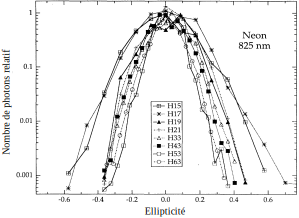
\includegraphics[width=0.6\columnwidth]{Figures/Polar/Intensity_f_ellipticity_budil}%
\caption{Intensité normalisée des harmoniques produites dans le néon en fonction de l'ellipticité. Tiré de \mycite{budilPRA1993}}%
\label{Fig:budil}%
\end{figure}
On observe une décroissance de l'intensité harmonique en fonction de l'ellipticité. Cet effet est marqué : on perd environ un ordre de grandeur en intensité quand $|\epsilon_{IR}| = 0.2$. On remarque également que cette décroissance est de plus en plus piquée lorsque l'ordre harmonique augmente.

\'{E}tudions ensuite les résultats de \mycite{AntoinePRA1997}. Les auteurs se sont cette fois intéressés à l'état de polarisation du rayonnement harmonique en fonction de l'ellipticité de l'infrarouge. Ces expériences ont été réalisées sur une version antérieure du système laser que nous avons utilisé dans la partie III. Pour caractériser le rayonnement, les auteurs mesurent des \textit{lois de Malus}, méthode optique qui sera présentée plus loin (section \ref{sec:resonant_argon_exp}). Comme on le verra, cette technique est incapable de mesurer le degré de polarisation $P$. Elle ne donne qu'une borne supérieure sur l'ellipticité, atteinte uniquement lorsque la lumière est complètement polarisée. Ce point est crucial dans le cas de la GHOE : comme expliqué dans la partie \ref{sec:introHHG}, le dipôle de chaque ordre harmonique dépend de l'intensité infrarouge. Le champ émis sera donc non homogène en polarisation spatialement et temporellement, donc nécessairement partiellement polarisé.

La figure \ref{fig:antoinepra} présente quelques résultats extraits de \mycite{AntoinePRA1997}. On y voit l'évolution de l'ellipticité des harmoniques et de l'angle d'orientation de l'ellipse par rapport à un axe de référence fixe, $\eta$. L'ellipticité mesurée n'étant qu'une borne supérieure de l'ellipticité vraie, on la note $\epsilon^{max}_q$. La figure \ref{fig:antoinepra} inclut un résultat numérique qui donne lui accès à $P$ et donne une idée de la quantité de lumière non-polarisée.

\begin{figure}[!ht]
\centering
\def\svgwidth{\columnwidth}
\import{Figures/Polar/}{antoinePRA.pdf_tex}
\caption{\`{A} gauche, mesure de l'ellipticité des harmoniques 17 et 23 générées dans l'argon par un champ infrarouge elliptique. Carrés rouges : mesures expérimentales de $\epsilon^{max}_q$ par loi de Malus. Comme expliqué plus haut, ce n'est qu'une borne supérieure sur la vraie valeur de l'ellipticité. En traits rouges, même quantité obtenue par le calcul. En pointillés noirs, véritable ellipticité obtenue par le calcul. En traits-pointillés verts, degré de polarisation obtenu par le calcul. \`{A} droite, mesure de l'angle de rotation de l'ellipse (carrés rouges) et même quantité obtenue par le calcul (traits rouges). Adapté de \mycite{AntoinePRA1997}.}
\label{fig:antoinepra}
\end{figure}

On fait les observations suivantes :
\begin{itemize}
\renewcommand{\labelitemi}{$\bullet$}
\setlength\itemsep{1em}
\item $\epsilon^{max}_q$ est une fonction croissante de $\epsilon_{IR}$ sur l'intervalle parcouru.
\item $|\epsilon^{max}_q|$ augmente plus rapidement avec $|\epsilon_{IR}|$ pour l'harmonique plus basse.
\item Le rayonnement est de moins en moins polarisé à mesure que $|\epsilon_{IR}|$ augmente. Cet effet est plus fort pour l'harmonique basse.
\item Cette diminution de $P$ s'accompagne d'une ellipticité vraie plus faible. Pour l'harmonique la plus basse, l'ellipticité vraie est presque \textit{deux fois inférieure} à l'ellipticité mesurée.
\item $\eta$ est également une fonction croissante de $\epsilon_{IR}$.
\item $\eta$ augmente plus rapidement pour l'harmonique basse.
\end{itemize}
\vspace{\baselineskip}
Ces deux travaux démontrent deux résultats généraux. En premier lieu, on voit que l'ellipticité de l'infrarouge est bien transférée au champ harmonique. Toutefois, l'ellipticité harmonique semble toujours rester inférieure à celle du laser générateur. Deuxièmement, le rendement harmonique décroît exponentiellement avec l'ellipticité de l'infrarouge. Nous concluons donc qu'il est très difficile d'obtenir un rayonnement ultraviolet d'ellipticité significative tout en gardant un niveau de signal suffisant. Dans la section suivante, nous expliquons les effets physiques à l'origine de ces propriétés.

\subsection{Description théorique de la GHOE en polarisation elliptique}
Dans le modèle à trois étapes (voir section \ref{sec:threestep}), la polarisation du champ intervient dans le calcul de la trajectoire électronique dans le continuum. On note $(x,y)$ la position dans le plan transverse de l'électron, que l'on considère classiquement. Sa trajectoire dans un champ complètement polarisé est donnée par :
\[\left\{
\begin{array}{l}
  \ddot{x}(t) = -\frac{qE_0}{m}\cos\omega t \\
  \ddot{y}(t) = -\epsilon\frac{qE_0}{m}\sin\omega t,
\end{array}
\right.\]
avec $q$ et $m$ la charge et la masse de l'électron, et $\epsilon$ et $\omega$ l'ellipticité et la fréquence angulaire du champ. L'équation selon $x$ se résoud exactement de la même façon que pour une polarisation linéaire : on suppose $x(t_i) = \dot{x}(t_i) = 0$, où $t_i$ est le temps d'ionisation, et pour chaque $t_i$, on obtient l'instant de recombinaison $t_r$.

Selon la dimension $y$, l'électron doit bien sûr être émis au niveau du noyau : $y(t_i) = 0$. Cependant, si on suppose que $\dot{y}(t_i) = 0$, l'équation $y(t_r) = 0$ n'a pas de solution : l'électron 'rate' l'atome et ne peut pas recombiner, comme illustré sur la figure \ref{fig:ellgruson}.

\begin{figure}[!ht]
\centering
\def\svgwidth{0.7\columnwidth}
\import{Figures/Polar/}{trajClassique.pdf_tex}
\caption{Trajectoire classique d'un électron dans un champ électrique elliptique, en supposant $x(t_i) = \dot{x}(t_i) = 0$ et $y(t_i) = \dot{y}(t_i) = 0$. La longueur d'onde est 800 nm et l'éclairement est $\SI{2e14}{W/cm^2}$. La polarisation du champ infrarouge est schématisée en gris. Adapté de \mycite{gruson}.}
\label{fig:ellgruson}
\end{figure}

Classiquement, la génération d'harmonique en polarisation elliptique est donc impossible. En vérité, le déplacement et la vitesse de l'électron selon l'axe $y$ sont trop faibles pour utiliser une description classique. Si on décrit cette dimension quantiquement, un paquet d'onde électronique est émis lors de l'ionisation tunnel. Ce paquet d'onde est localisé spatialement autour de l'atome, sur une longueur $\Delta y$ dépendant de l'orbitale en jeu. Le moment cinétique selon $y$ est donc lui aussi confiné à une largeur $\Delta p_y$. La distribution de $p_y$ est centrée sur 0 à $t=0$ et peut maintenant contenir des valeurs non nulles. \mycite{strelkov2006} démontre que pour avoir recombinaison, le moment cinétique initial doit valoir $p_y(t=0) = -\bar{y}/\tau$, où $\bar{y}$ est la quantité représentée sur la figure \ref{fig:ellgruson}, et $\tau$ le temps d'excursion total de l'électron. Ceci permet d'expliquer simplement le résultat de \mycite{budilPRA1993} présenté plus haut : si $\epsilon_{IR}$ augmente, $\bar{y}$ augmente également. Il faut donc un moment cinétique initial plus important pour avoir recombinaison, ce qui est moins probable puisque la distribution de $p_y(0)$ est centrée en 0. Ceci explique la diminution du rendement harmonique avec l'ellipticité de l'infrarouge.

Pour comprendre qualitativement les résultats de \mycite{AntoinePRA1997}, on trace les trajectoires classiques de l'électron, cette fois avec la condition initiale $p_y(0) = -\bar{y}/\tau$ et avec les deux trajectoires quantiques.

\begin{figure}[!ht]
\centering
\includegraphics[width=0.9\columnwidth]{Figures/Polar/higuet.png}%
\caption{Trajectoires électroniques correspondant à l’harmonique 111 d'un laser à 1800 nm, pour un éclairement de $\SI{1e14}{W/cm^2}$ et une ellipticité de 0.2 (champ représenté en gris).
En ligne pointillée, la direction du champ à l’instant d’ionisation. On notera la différence entre les échelles
des axes $x$ et $y$. Tiré de \mycite{higuet}}
\label{fig:ellhiguet}%
\end{figure}

La figure \ref{fig:ellhiguet}, tirée de \mycite{higuet}, n'est pas directement comparable à la figure \ref{fig:ellgruson}, le calcul ayant été réalisé à une longueur d'onde plus élevée. Une longueur d'onde plus grande conduit à des trajectoires électroniques plus longues et à des effets plus marqués qu'à 800 nm.
On observe toutefois un effet intéressant : l'électron recombine sur l'atome avec un angle variable $\beta_{c/l}$. Cette angle est responsable de la rotation de l'ellipse harmonique d'angle $\eta$. En effet, pour une orbitale de symétrie sphérique, l'axe principal de l'ellipse de polarisation du rayonnement harmonique est dirigé selon la direction de recollision de l'électron à la recombinaison \mycite{strelkov2006}. L'ellipse harmonique est donc tournée d'un angle $\beta_{c/l}\approx\eta$, qui dépend de l'ordre harmonique et de la trajectoire considérée. On remarque que $\beta_c$ et $\beta_l$ sont de signes différents, la dépendance de $\eta$ est donc de signe opposé pour la trajectoire longue. Ceci peut être mesuré expérimentalement (voir e.g. la figure 3.11 de \mycite{higuet}).\par
Enfin, cet angle explique également que le rayonnement harmonique soit elliptique. L'argument donné par \mycite{Strelkov2011} est le suivant : on considère un état lié $\psi_0(x,y,z) = \psi(x)\psi(y)\psi(z)$ et un paquet d'onde électronique. Ce paquet se déplace principalement dans la direction $x$ et possède une amplitude dans les deux autres dimensions : $\chi(x,y,z) = f(y,z)\exp(\rmi p_x x)$. Comme on l'a vu, l'amplitude $f(y,z)$ est initialement centrée en $y=0$ puis se décale selon $y$ au cours de la propagation. \`{A} la recombinaison, on peut faire un développement de Taylor de $f$ : $f(y,z) = f_0 + f_1 y$, où $f_1$ est relié à l'angle de recombinaison. Le moment dipolaire du système vaut 
\[\bm{d} = \int{\psi_0^* \bm{r} \chi \rmd\bm{r}} + \text{c.c.}\]
On obtient donc ses composantes cartésiennes :
\[d_x \propto f_0 \text{  et  } d_y \propto \rmi f_1.\]
On excite donc un dipôle dans les deux directions transverses, et leurs oscillations sont décalées de $\pi/2$. Le signal émis est donc polarisé elliptiquement.

\section{Méthodes existantes de génération d'harmoniques elliptiques}
Dans la partie précédente, nous avons expliqué le mécanisme de GHOE en polarisation elliptique et vu que le processus ne permettait pas un transfert direct et efficace de l'ellipticité de l'infrarouge vers l'ultraviolet. Nous présentons ici trois méthodes existantes pour circonvenir à ce problème. 

\subsection{Réflexion sur des surfaces métalliques}
\label{sec:metalsurface}
L'idée est ici de générer des harmoniques polarisée linéairement puis d'utiliser un dispositif similaire à une lame quart d'onde. Dans ces gammes spectrales, il est impossible de réaliser une lame quart-d'onde conventionnelle, mais on peut obtenir le même effet à partir de plusieurs surfaces métalliques. \par
On appelle plan d'incidence le plan formé par le vecteur d'onde du champ incident et le vecteur normal à la surface. Il est alors courant d'appeler $p$ la composante du champ \textit{parallèle} à ce plan et $s$ la composante perpendiculaire (\textit{senkrecht} en allemand). Selon le métal utilisé, ces deux composantes ne sont pas réfléchies également : la surface métallique présente une réflectivité selon chaque dimension, habituellement notées $R_p$ et $R_s$. De plus, elle introduit un déphasage entre ces deux composantes. Il est ainsi possible d'introduire un déphasage de $\pi/2$ en choisissant une bonne combinaison de miroirs. \mycite{VodungboOE2011} ont développé un dispositif à 4 miroirs de Mo/$\text{B}_\text{4}$C qui permettent d'obtenir les harmoniques 31 à 45 avec une ellipticité variant de 1 à 0.61. Ces caractéristiques sont très intéressantes, malgré un inconvénient majeur : la transmission du dispositif varie entre 2.6 et 3.7 \% sur la plage considérée. Ce type de dispositif a continué à être amélioré, \mycite{WillemsPRB2015} reportent par exemple une transmission de 10-30\% et une ellipticité de $\approx 0.8$ entre 45 et 70 eV.\par

Ces dispositifs sont assez difficiles à implémenter, ce qui couplé à leur faible transmission explique qu'ils ne soient pas très répandus aujourd'hui. 

\subsection{Génération dans des molécules alignées}
Considérons la GHOE avec un faisceau polarisé linéairement, cette fois dans un gaz de molécules diatomiques. Au niveau microscopique, l'orientation de l'axe de la molécule par rapport à la polarisation du laser joue un rôle crucial : l'angle de recombinaison de l'électron par rapport à cet axe modifie l'émission, exactement comme le champ elliptique représenté sur la figure \ref{fig:ellhiguet}. L'électron peut donc exciter les deux composantes du dipôle. L'interprétation est toutefois plus compliquée, puisque l'ellipticité obtenue dépend de la symétrie de ou des orbitales ionisées, de leur phases relatives ou encore de l'intensité de génération (voir \mycite{MairessePRL2010}). \par
\`{A} l'échelle macroscopique, toutes les orientations de molécules par rapport au laser sont équiprobables. On a donc un effet de moyenne, qui donne un rayonnement harmonique macroscopique polarisé linéairement. Il faut donc \textit{aligner} les molécules. Une technique courante est l'alignement impulsionnel, qui utilise une pré-impulsion quelques secondes avant l'impulsion de génération \mycite{RoscaPRL2001}. La figure \ref{fig:n2ell} présente deux exemples de résultats obtenus avec $\text{N}_\text{2}$, tirés de \mycite{ZhouPRL2009} et \mycite{MairessePRL2010}. Dans les deux cas, on observe un maximum d'ellipticité pour l'harmonique 23 et pour un angle d'alignement d'environ 60\degres.

\begin{figure}[!ht]
\centering
\def\svgwidth{1\columnwidth}
\import{Figures/Polar/}{n2ell.pdf_tex}
\caption{Mesures d'ellipticité en fonction de l'ordre harmonique et de l'angle d'alignement des molécules de $\text{N}_\text{2}$ par rapport à la polarisation du laser. \`{A} gauche, résultat tiré de \mycite{ZhouPRL2009}, où I = $\SI{2e14}{W/cm^2}$. \`{A} droite, résultat tiré de \mycite{MairessePRL2010}, où I = $\SI{8e13}{W/cm^2}$. Les ellipticités mesurées ici sont des bornes supérieures et non pas la vraie valeur.}
\label{fig:n2ell}
\end{figure}

Ce résultat s'explique en fait par la présence de plusieurs canaux d'ionisation et est donc très intéressant du point de vue de la spectroscopie harmonique. Il est toutefois assez peu flexible et nécessite d'aligner des molécules, et fournit de plus une ellipticité modeste. De plus, l'utilisation d'une impulsion d'alignement a tendance à créer davantage d'inhomogénéités spatiales et temporelles, ce qui produit un rayonnement peu polarisé. Cette question est étudiée en détail expérimentalement dans la thèse de Vincent Gruson \mycite{gruson}.

\subsection{Manipulation de la trajectoire électronique par un champ bicolore}
Terminons par la méthode la plus récente, qui est peut-être la plus intuitive. Le principe est ici de contrôler optiquement la trajectoire électronique de sorte à ce que la recombinaison soit possible quelque soit l'ellipticité infrarouge. Une solution à ce problème a été initialement donnée par \mycite{EichmannPRA1995}. En utilisant un champ à deux couleurs d’ellipticités opposées et de deux longueurs d'onde commensurables, par exemple 400 et 800 nm, la GHOE est possible. L'expérience réalisée par \mycite{FleischerNP2014} montre que la génération est efficace dans ces conditions, et permet de générer des harmoniques paires et impaires d'ellipticité $|\epsilon^{max}_q|\approx 1$. \mycite{KfirNP2015} a mesuré l'hélicité (le signe de $\epsilon$) et montré que les ordres harmoniques étaient polarisés ainsi:
\[\left\{
\begin{aligned}
  \text{Si }q&=3m-1,\quad &\epsilon_q \approx \pm 1 \\
	&=3m+1, &\epsilon_q \approx \mp 1 \\
	&=3m, &\text{l'harmonique n'est pas générée},
\end{aligned}
\right.\]
où $\pm$ dépend de l'hélicité des champs générateurs. Cette méthode est très intéressante car elle produit un rayonnement fortement polarisé et intense. Elle a été utilisée avec succès par \mycite{KfirNP2015} pour réaliser des mesures de dichroïsme circulaire magnétique dans le cobalt, un effet voisin de ceux dont il sera question au chapitre \ref{sec:PECD}. Cette méthode est ainsi particulièrement adaptée à la spectroscopie de solides.\par
La réponse d'une molécule est quant à elle plus difficile à interpréter. En effet, un grand nombre de degrés de liberté et différents canaux d'ionisation contribuent au spectre total, et il n'est jamais facile d'identifier chacune de ces contributions. 
On préférera donc avoir un rayonnement très simple, de sorte à exciter le moins d'effets possibles et de pouvoir les identifier. La technique présentée ici fournit un spectre harmonique dense fait d'harmoniques paires et impaires d'hélicité en alternance, ce qui est à l'opposé des besoins de la spectroscopie moléculaire.

\section{Polarisations elliptiques produites par GHOE résonante}
Nous présentons ici notre méthode pour produire un rayonnement ultraviolet polarisé elliptiquement. Cette source a été développée pour être utilisée dans l'étude de la photoionisation de molécules. Ces travaux, ainsi que la totalité du reste de ce chapitre, ont été réalisés au CELIA Bordeaux en collaboration avec l'équipe de Yann Mairesse. Les résultats correspondant aux parties XX à XX ont été publiées dans \mycite{FerreNP2015}, Article N inclus dans cette thèse.

L'idée ici est de modifier la dynamique électronique dans la GHOE non pas en structurant le champ laser, mais en utilisant le potentiel de la molécule lui-même. En particulier, ce potentiel peut être structuré par la présence de \textit{résonances}. Ces phénomènes ont été très largement étudiés dans le cadre de la photoionisation, et se manifestent en général par une augmentation de la section efficace d'absorption pour une énergie de photon précise. Cette énergie résonante coïncide avec l'énergie nécessaire à un des canaux d'ionisation de la molécule, ce qui ouvre ce canal et augmente la section efficace en lien avec la force d'oscillateur de cette transition. De nombreux mécanismes sont connus et documentés par des études réalisées sur synchrotron, peuvent impliquer un ou plusieurs électrons, ou encore apparaître en dessous ou au dessus du seuil d'ionisation.

La photoionisation est le processus conjugué à la recombinaison radiative. Il est donc naturel que des effets des résonances moléculaires soient visibles en GHOE, où la recombinaison joue un rôle central. Une résonance peut avoir des effets très variés sur la GHOE. L'étape résonante peut être soit l'ionisation, par exemple dans le cas d'une résonance multiphotonique \mycite{AckermannOE2012,ChuPRA2013}, soit à la recombinaison, qui peut être magnifiée par une résonance de forme ou par un piégeage dans un état de Rydberg \mycite{TaeibPRA2003,TudorovskayaPRA2011}. La présence d'une résonance empêche souvent de réaliser l'approximation de champ fort et met en défaut le modèle à trois étapes \mycite{StrelkovPRL2010}. Commençons par étudier le cas de l'argon.

\subsection{Génération résonante dans l'argon : cas des résonances sous le seuil}
\subsubsection{Mécanismes résonants autour du seuil}
La figure \ref{fig:ArIp} montre la section efficace de photoabsorption de l'argon. On y voit une série de pics d'absorption en dessous du seuil d'ionisation, qui correspondent aux états de Rydberg de l'atome.

\begin{figure}[!ht]
\centering
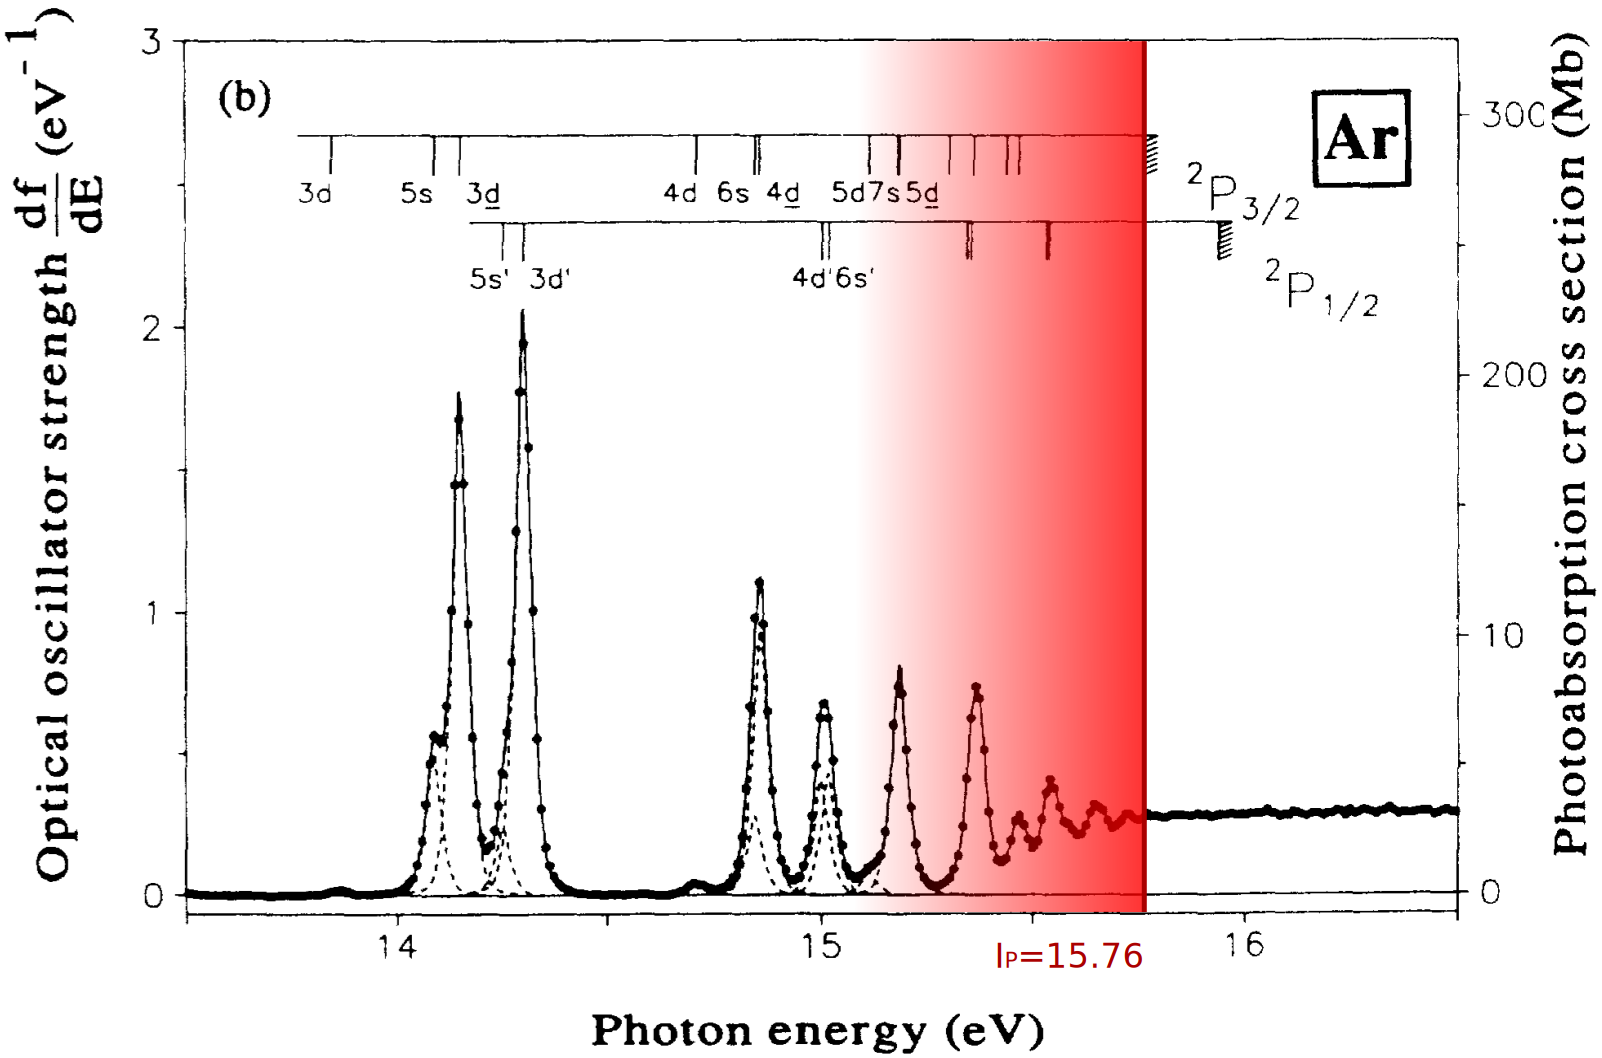
\includegraphics[width=0.9\columnwidth]{Figures/ResonantArgon/argon_spectrum.png}%
\caption{Section efficace de photoabsorption de l'argon dans la gamme 13.5-16.5 eV. Les lignes pointillées correspondent aux pics déconvolués. Tiré de \mycite{ChanPRA1992}.}
\label{fig:ArIp}%
\end{figure}

Nous allons voir que cette structure bien particulière donne lieu à plusieurs phénomènes intéressants. L'argon est un système de choix car son potentiel d'ionisation ($I_p = \SI{15.76}{eV}$) est très proche de l'énergie de 10 photons d'un laser Ti:Sa ($10\times 1.55 = 15.5$ eV). L'étude de la GHOE au voisinage du potentiel d'ionisation a été réalisée expérimentalement par \mycite{ChiniNP2014}, qui observèrent une émission à la fois en dessous et au dessus du seuil. Cette émission semble avoir des caractéristiques inhabituelles par rapport à la GHOE classique. En particulier, les auteurs remarquent une augmentation du signal avec la pression sans observer de phénomène de saturation, mais n'expliquent pas le mécanisme sous-jacent. Ensuite, \mycite{XiongPRL2014} et surtout \mycite{CampPRA2015} expliquent ce mécanisme en détail et montrent qu'il est lié à la présence des états de Rydberg de la figure \ref{fig:ArIp}. Deux effets distincts interviennent dans la génération.

Le premier est un mécanisme de GHOE résonante ayant lieu pendant l'ionisation de l'atome. Pendant la durée du pulse, tous les niveaux énergétiques de l'atome sont décalés par effet Stark. Pour les états de Rydberg de la figure \ref{fig:ArIp}, ce décalage vaut environ $U_p$, l'énergie pondéromotrice \mycite{GaardePRA2001,FiguieraPRA2002}. Ainsi, l'énergie d'un de ces niveaux peut devenir égale à l'énergie de $n$ photons infrarouges (dans notre cas, $n=10$). On a alors une résonance multi-photonique, qui augmente drastiquement l'intensité de la $n$-ième harmonique. La condition de résonance s'écrit : $n\hbar\omega = |E_R-E_0|+U_p$, où $E_R$ et $E_0$ sont respectivement les énergies de l'état fondamental et de l'état de Rydberg. Ce phénomène était déjà connu en ionisation au-dessus du seuil (ATI pour \textit{Above Threshold Ionization}) avec des impulsions courtes \mycite{FreemanPRL1987,AgostiniPRL1989}. On remarquera que pour l'argon, l'ordre harmonique résonant est le 10ème, qui n'est pas généré dans les conditions habituelles. Pour observer cet effet, on utilisera donc soit des impulsions infrarouges très courtes, soit on choisira une autre longueur d'onde de génération. Dans la suite, nous utiliserons une longueur d'onde de 400 nm, pour laquelle on a une résonance à 5 photons au seuil de l'argon.

Le second effet ne correspond pas à la GHOE, mais produit quand même un rayonnement ultraviolet dans cette région. Dans ce mécanisme, le faisceau infrarouge crée une superposition d'état cohérente entre l'état fondamental d'énergie $E_0$ et quelques états de Rydberg d'énergie $E_R$, via une transition multiphotonique. Le dipôle ainsi créé émet une radiation d'énergie $E_R-E_0$ pendant une durée correspond à la durée de vie de l'état de Rydberg, c'est-à-dire bien plus longtemps que l'émission harmonique. Ce rayonnement a donc une structure spectrale très fine. Ce processus s'appelle \textit{Free Induction Decay} ultraviolet (xFID) \mycite{BengtssonLarsenEtAl2015}, et était déjà connu en Résonance Magnétique Nucléaire \mycite{BlockPR1946} et dans l'infrarouge \mycite{BrewerPRA1972}. 

L'influence de ces deux effets a été étudiée expérimentalement en détail au CELIA Bordeaux par \mycite{beaulieuArXiv2016}. Des expériences réalisées à 800 nm ont permis d'observer les rayonnements issus de chacun de ces deux effets et d'étudier leurs propriétés de cohérence temporelle. Un spectre typique obtenu avec une impulsion de 7 fs est présenté sur la figure \ref{fig:xFID}. Les auteurs démontrent également la possibilité d'avoir ionisation à partir d'un état de Rydberg excité et recombinaison sur l'état fondamental, ce qui donne l'émission pointée par la ligne violette sur la figure \ref{fig:xFID}. 

\begin{figure}[!ht]
\centering
\includegraphics[width=1.1\columnwidth]{Figures/ResonantArgon/xFID.pdf}%
\caption{Spectre obtenu dans l'argon avec une impulsion de 7 fs à 800 nm. L'intensité est de $\SI{5.2e13}{W/cm^2}$. On observe le rayonnement xFID en dessous du seuil d'ionisation, que l'on compare avec le spectre d'absorption tiré de la figure \ref{fig:ArIp}. Ensuite, on observe les harmoniques non résonantes (lignes verticales bleues) ainsi que celles provenant d'états de Rydberg excités (lignes verticales violettes). Tiré de \mycite{beaulieuArXiv2016}.}
\label{fig:xFID}
\end{figure}

L'effet xFID est également très intéressant fondamentalement et permet de mesurer des observables similaires à celles obtenue en spectroscopie d'absorption transitoire attoseconde (ATAS, pour \textit{Attosecond Transient Absorption Spectroscopy}) \mycite{BeckNJP2014}. En collaboration avec Samuel Beaulieu, \'{E}tienne Bloch, Valérie Blanchet et Yann Mairesse, nous avons étudié ce point expérimentalement, cette fois avec une longueur d'onde de 400 nm et en choisissant des conditions de focalisation favorisant grandement le xFID. Ces expériences sont en cours d'analyse et ne seront pas présentées dans ce manuscrit. Nous nous intéressons maintenant à la polarisation du rayonnement au voisinage du seuil d'ionisation.

\subsubsection{Ellipticité du rayonnement près du seuil de l'argon}
\label{sec:resonant_argon_exp}
Pour avoir une résonance multiphonique au seuil de l'argon, nous choisissons de travailler à 400 nm. L'utilisation de cette longueur d'onde a deux autres avantages : (1) La GHOE est plus efficace, l'efficacité évolue en effet en $\lambda^{\simeq-6}$ \mycite{ShinerPRL2009}. (2) La largeur spectrale entre chaque harmonique est doublée et l'énergie de coupure diminue, on aura donc très peu d'harmoniques. Comme on le verra, ceci est très favorable dans les expériences de dichroïsme circulaire présentées plus loin. 

Ces expériences et toutes celles qui vont suivre ont été réalisées sur le système Aurore du CELIA Bordeaux, qui délivre des impulsions de 8mJ, 25 fs à environ 800 nm et à un taux de répétition de 1 kHz. Ce faisceau est ensuite doublé en fréquence par un BBO de type 1 et de $\SI{200}{\micro\meter}$ d'épaisseur. On mesure qu'à partir de 4 mJ du fondamental, on obtient 1 mJ à 404 nm. Le 800 nm restant est filtré à l'aide de miroir dichroïques, tandis que le 400 nm est focalisé par une lentille mince de Si$\text{O}_\text{2}$ de 50 cm de focale. Le reste du dispositif est similaire à celui présenté sur la figure \ref{Fig:ExpG} : des harmoniques sont générées dans un jet de gaz continu (ouverture de $\SI{300}{\micro\meter}$) puis imagées par un réseau de diffraction couplé à une galette de micro-canaux. 

Dans ce dispositif de GHOE assez typique, nous souhaitons rajouter une mesure de l'état de polarisation du rayonnement. Nous choisissons de mesurer des \textit{loi de Malus}. Habituellement, ces lois sont obtenues en mesurant l'intensité transmise par un polariseur parfait en fonction de l'angle du polariseur $\theta_p$ par rapport au champ électrique. Si le champ électrique est polarisé linéairement, l'intensité sera totalement transmise lorsque le polariseur est orienté parallèlement à la direction de polarisation du champ, et non transmise s'il est orthogonal. A contrario, si le champ est circulaire, l'intensité transmise ne variera pas en fonction de $\theta_p$. De manière générale, on obtient un signal oscillant de la forme 
\[I(\theta_p) = \epsilon^2+(1-\epsilon^2)\cos^2(\eta-\theta_p),\]
où $\epsilon$ et $\eta$ ont été définis dans la partie \ref{sec:polardef}. Remarquons que ce type de mesure est insensible à la partie non polarisée de la lumière, dont la contribution ne dépendant pas de $\theta_p$. Ainsi, la valeur d'$\epsilon$ mesurée ici est encore une fois uniquement une borne supérieure, $\epsilon^{max}$. On voit donc que seulement pour une onde totalement polarisée, la mesure d'une loi de Malus donne accès à tous les paramètres de Stokes, définis plus haut. 

Il reste donc à réaliser un polariseur pour le rayonnement harmonique. Nous avons déjà mentionné que les surfaces métalliques présentaient des réflexions $R_s$ et $R_p$ différentes selon chaque dimension transverse (voir section \ref{sec:metalsurface}). Ainsi, en utilisant plusieurs de ces surfaces à la suite, on peut quasiment filtrer la composante $s$ ou $p$. Nous choisissons d'utiliser trois miroirs avec revêtement en or placés à 75\degres-60\degres-75\degres, ce qui donne un rapport total $R_s/R_p$ valant 5 à 20 pour la gamme spectrale étudiée. Enfin, plutôt que de motoriser et de faire tourner ce polariseur sous vide, on préfère tourner l'orientation du champ de génération et garder le polariseur fixe, ce qui est équivalent. Ce polariseur imparfait doit être pris en compte dans l'analyse de la loi de Malus (voir \mycite{AntoinePRA1997} ainsi que \mycite{gruson}), mais n'empêche pas de mesurer les paramètres recherchés, comme l'illustre la figure \ref{fig:malus} pour l'harmonique 5. Pour plus de détail sur ce dispositif de polarimétrie harmonique on se reportera à la thèse d'Amélie Ferré \mycite{ferre}.

\begin{figure}[!ht]
\centering
\def\svgwidth{0.7\columnwidth}
\import{Figures/ResonantArgon/}{malus.pdf_tex}
\caption{Lois de Malus pour l'harmonique 5 du faisceau à 404 nm. On mesure l'intensité transmise par le polariseur XUV en fonction de la direction de polarisation du champ de génération, lorsqu'il est polarisé linéairement (rouge) ou elliptiquement (vert). On voit que le champ harmonique est maximal en $\theta_p = \eta$, ce qui donne la direction de son ellipse de polarisation. Par ailleurs, on observe une diminution du contraste des oscillations avec $\epsilon_{IR}$, signe d'une ellipticité harmonique plus élevée. L'analyse des oscillations donne ici $\epsilon_q^{max} \simeq 0.6$ quand $\epsilon_{IR}=0.287$.}
\label{fig:malus}
\end{figure}

La figure \ref{fig:resonant_argon_exp} présente les résultats obtenus lorsque le laser de génération porte une ellipticité $\epsilon_{IR} = 0.4$. On observe les harmoniques 5, 7 et 9 du fondamental à 404 nm. Les harmoniques 7 et 9 présentent un profil gaussien spectralement, tandis que l'harmonique 5 est structurée. Cette structure est due au xFID, effet présenté plus haut. Le rayonnement xFID est superposé à l'émission harmonique, qui est résonante due à la résonance à 5 photons.  On mesure ensuite l'ellipticité en fonction de l'énergie de photon. On voit que l'ellipticité apparente des harmoniques non résonantes est de l'ordre de $\epsilon_{IR}$, tandis que celle de l'harmonique résonante est presque doublée (valeur maximale de 0.77).  

\begin{figure}[!ht]
\centering
\def\svgwidth{1\columnwidth}
\import{Figures/ResonantArgon/}{exp_result.pdf_tex}
\caption{Mesure d'ellipticité dans l'argon près du seuil d'ionisation. Le laser à 404 nm a une ellipticité de $\epsilon_IR=0.4$. Sur l'échelle de gauche (bleue), intensité en fonction de l'énergie de photon. On observe trois harmoniques, desquelles on mesure l'ellipticité apparente. On obtient les courbes rouges, échelle de droite.}
\label{fig:resonant_argon_exp}
\end{figure}

Pour confirmer que cette forte ellipticité est due à la présence de résonances, Bernard Pons et Baptiste Fabre, du CELIA Bordeaux, ont réalisé une étude théorique du problème. On résout l'équation de Schrödinger dépendante du temps (TDSE, \textit{Time-Dependant Schrödinger Equation}) à deux dimensions, en utilisant un potentiel de Coulomb de "`cœur mou"', qui reproduit la présence du potentiel d'ionisation et des états sous-jacents. La figure \ref{fig:resonant_argon_th_bound} illustre ce potentiel ainsi que le spectre harmonique obtenu. On observe des structures spectrales similaires à l'expérience, à la fois dans l'intensité et dans l'ellipticité de l'harmonique 5. L'ellipticité est en particulier très modulée, mais ne prend pas des valeurs aussi élevées que celles mesurées. Au contraire, elle devient même négative à 14 eV. Les calculs ont été répétés et ont permis d'observer qu'une très légère modification du potentiel atomique donnaient lieu à de très fortes modifications de l'ellipticité. On s'attend donc à n'avoir qu'un accord qualitatif.

\begin{figure}[!ht]
\centering
\def\svgwidth{1\columnwidth}
\import{Figures/ResonantArgon/}{th_result_bound.pdf_tex}
\caption{Résultat théorique en utilisant un potentiel de Coulomb de cœur mou. En haut, on représente le profil de ce potentiel, qui peut être ajusté pour obtenir la bonne valeur d'$\text{I}_{\text{p}}$. En bas, mêmes grandeurs que celles mesurées expérimentalement sur la figure \ref{fig:resonant_argon_exp}.}
\label{fig:resonant_argon_th_bound}
\end{figure}

En conclusion, nous voyons que la présence de résonances sous le seuil induit une modulation de l'ellipticité. Nous mesurons de plus qu'elle augmente très fortement. On obtient donc un rayonnement aux propriétés intéressantes sans véritable perte de signal : une mesure par une photodiode calibrée montre que l'harmonique 5 contient $\num{7e6}$ photons par impulsion. De plus, le caractère résonant de l'harmonique 5 fait qu'elle ne subit pas d'effet de réabsorption \mycite{ChiniNP2014}. Son flux peut donc être facilement augmenté par une pression de génération plus élevée.  Toutefois, cette méthode est restreinte à des énergies de photons relativement basses, correspondant au seuil d'ionisation du gaz utilisé. Les gaz habituellement utilisés pour avoir un flux important sont l'argon, $\text{I}_{\text{p}}=15.76$ eV, le krypton, $\text{I}_{\text{p}}=14$ eV, ou le xénon, $\text{I}_{\text{p}}=12.13$ eV. Il serait donc intéressant de généraliser notre approche à d'autres résonances d'énergie plus élevée. Dans la section suivante, nous étudions le cas de résonances dans le continuum.

\subsection{Génération autour d'une résonance dans le continuum}
Ces résonances se manifestent de la même façon que celles présentées plus haut : une augmentation de la section efficace de photoionisation. Nous nous intéressons au cas des \textit{résonances de forme} \mycite{Dehmer1972}, couramment observées dans le spectre de petites molécules. Bien qu'elles aient été observées assez tôt, leur interprétation et leur définition fait régulièrement débat, comme en témoigne l'article de \mycite{Piancastelli1999}, intitulé "\textit{The neverending story of shape resonances}" . Une interprétation courante est la suivante. Ces résonances sont dues à une barrière présente dans le potentiel moléculaire. Cette barrière est la résultante de forces attractives (e.g. coulombienne) et répulsives (effets d'écrantage, force centrifuge). Quand un photoélectron possède l'énergie correspond à cette barrière, il se retrouve dans un état métastable \mycite{simons1984roles}, piégé dans la barrière de potentiel, dont il finit par s'échapper par effet tunnel. La figure \ref{fig:shaperesonance} illustre ce principe : à l'énergie résonante, la fonction d'onde électronique est localisée sur le puit central et temporairement piégée.

\begin{figure}[!ht]
\centering
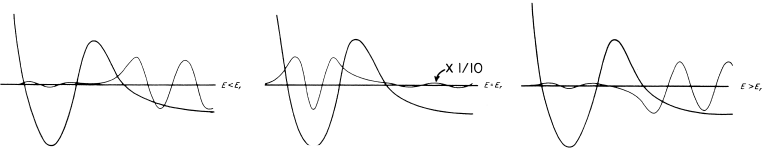
\includegraphics[width=1\columnwidth]{Figures/ResonantArgon/shape_resonance.pdf}%
\caption{Principe d'une résonance de forme. De gauche à droite, $E<E_r$, $E=E_r$ et $E>E_r$, où $E$ et $E_r$ sont les énergies du photoélectron et de la résonance. Tiré de \mycite{Piancastelli1999}.}
\label{fig:shaperesonance}
\end{figure}

De par sa nature, cette barrière de potentiel se situe relativement proche de la molécule. L'électron est ainsi spatialement localisé, ce qui augmente la densité électronique et produit en général un signal de photoionisation intense. Un autre intérêt de ces résonances et que la présence d'une barrière est liée à la forme de la molécule, d'où son nom. Ainsi, de nombreux travaux ont essayé de relier l'énergie des résonances de forme aux longueurs de liaisons de molécules adsorbées, méthodes astucieusement baptisées "\textit{Bond length with a ruler}" \mycite{StohrPRL1984}.

Nous étudions ici cet effet en ajoutant une barrière au potentiel de la figure \ref{fig:resonant_argon_th_bound} pour induire une résonance de forme vers l'énergie de l'harmonique 7. Ce potentiel ne correspond pas forcément à un système physique, mais nous permet de démontrer l'effet de la résonance du continuum. Le spectre obtenu est présenté sur la figure \ref{fig:resonant_argon_th_bound}. On y voit le potentiel choisi, ainsi que la position de la résonance de forme. En orange, on représente une seconde résonance assez large du continuum, apparue après la modification du potentiel.

\begin{figure}[!ht]
\centering
\def\svgwidth{1\columnwidth}
\import{Figures/ResonantArgon/}{th_result_continuum.pdf_tex}
\caption{Résultat théorique en utilisant un potentiel de Coulomb de cœur mou auquel on ajoute une barrière. Le potentiel est représenté en haut de la figure. La ligne turquoise indique la position de la résonance de forme, tandis que la zone orange est une résonance large dans le continuum également apparue après modification du potentiel. En bas, mêmes grandeurs que celles mesurées expérimentalement sur la figure \ref{fig:resonant_argon_exp}.}
\label{fig:resonant_argon_th_continuum}
\end{figure}

Nous voyons donc que l'ellipticité de l'harmonique 7 et 9 sont significativement augmentés par la présence des deux résonances. La relation entre résonance et haute ellipticité est donc générale, ce qui permet de générer un rayonnement elliptique dans de nombreuses gammes énergétiques. Comment maintenant comprendre physiquement l'augmentation de cette ellipticité ? \mycite{StrelkovPRL2010} décrit théoriquement la GHOE près d'une résonance d'autoionisation, qui apparaît également lorsque le potentiel présente une barrière. Il montre que le modèle à trois étape habituel doit être modifié : au moment de la recombinaison, l'électron est piégé par la barrière de potentiel, le système se retrouve donc dans un état résonant du même type que celui de la figure \ref{fig:shaperesonance} avant de finalement se relaxer vers l'état fondamental en émettant un rayonnement XUV. Ce processus explique l'augmentation du signal harmonique près de la résonance par une forte section efficace de diffusion inélastique (qui contrôle le peuplement de l'état résonant) ainsi qu'une forte force d'oscillateur pour la transition entre l'état résonant et l'état fondamental.
Cette interprétation est tout à fait analogue à celle d'une résonance de forme en photoionisation donnée plus haut, ce qui illustre bien le caractère conjugué de ces deux effets.

Pour vérifier que l'ellipticité est bien créée par cette étape de piégeage, Bernard Pons et Baptiste Fabre ont effectué des calculs TDSE au moment de la recombinaison. On s'intéresse au paquet d'onde électronique d'abord ionisé, qui se propage puis recombine sur l'état fondamental. Le potentiel est le même que celui présenté sur la figure \ref{fig:resonant_argon_th_continuum}. Ce paquet d'onde $\Psi(\bm{r},t)$ se décompose sur une base d'états propres de l'hamiltonien du système (voir Supplementary Information de l'article XX pour plus de détails) :
\[ \Psi(\bm{r},t)=\sum_{E_n>0,l} a_{E_n,l}^{(o,e)}(t)\phi_{E_n,l}^{(o,e)}(\bm{r})e^{-(\rmi E_n t)},\]
où $\phi_{E_n,l}^{(o,e)}$ est l'état propre d'énergie $E_n$, positive puisqu'on cherche les électrons dans le continuum, de moment angulaire $l$, et $a_{E_n,l}^{(o,e)}$ est l'amplitude. $(o,e)$ correspondent à la symétrie de l'état par rapport à l'axe $\bm{e_x}$. Si on considère la recombinaison sur un état fondamental de symétrie $s$, seulement $\phi_{E_n,1}^{e}$ et $\phi_{E_n,1}^{o}$ contribuent. Ils correspondent respectivement à l'état propre parallèle $p_x$ et perpendiculaire $p_y$. La probabilité de trouver l'électron dans un de ces états est $P_{x,y}(E_n,t) = |a_{E_n,l}^{(o,e)}(t)|^2$. On choisit $E_n$ proche de l'énergie de résonance et on considère des instants proches de l'instant de recombinaison correspondant à l'harmonique 7. Les probabilités $P_x$ et $P_y$ sont représentées sur la figure \ref{fig:resonant_proba}.

\begin{figure}[!ht]
\centering
\def\svgwidth{1\columnwidth}
\import{Figures/ResonantArgon/}{electron_dynamics_resonance.pdf_tex}
\caption{\'{E}volution temporelle des probabilités $P_x$ (tirets bleus) et $P_y$ (traits pleins rouges) du paquet d'onde électronique arrivant sur un système présentant une résonacne de forme. Le champ électrique a un cycle optique à 400 nm, une intensité pic de $\SI{10e14}{W/cm^2}$ et une ellipticité de 0.3.}
\label{fig:resonant_proba}
\end{figure}

Nous observons que la probabilité perpendiculaire $P_y$ augmente graduellement, jusqu'à dépasser $P_x$. Ceci signifie que la résonance de forme modifie géométriquement le paquet d'onde électrique alors qu'il s'approche de l'atome. Cette augmentation de $P_y$ se manifeste dans la GHOE par une augmentation de la composante perpendiculaire du champ émis et donc de son l'ellipticité.

\subsection{Application à la molécule de \sf6}
Nous appliquons maintenant le résultat obtenu expérimentalement. L'équipe du CELIA Bordeaux a étudié en détail la génération d'harmoniques dans un gaz de molécules de \sf6 (hexafluorure de soufre). Cette molécule a une structure octaédrique avec l'atome de soufre en son centre. Le panneau du haut de la figure \ref{fig:sf6_cross_section} montre la section efficace de photoionisation de \sf6. Le canal noté C correspond à une résonance d'autoionisation \mycite{fano1968}, tandis que le canal noté A est une résonance de forme. Un calcul numérique donne la contribution de ces canaux à la GHOE (panneau du bas), qui permet de voir que la génération autour des ordres 15 à 19 est dominée par ces deux canaux. On s'attend donc à avoir un transfert efficace d'ellipticité dans cette région spectrale.

\begin{figure}[!ht]
\centering
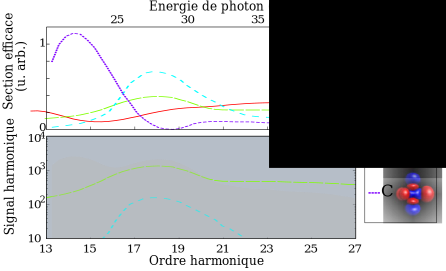
\includegraphics[width=.8\columnwidth]{Figures/SF6/sf6_cross_section.png}%
\caption{(Haut) Section efficace de photoionisation XUV de différents canaux d'ionisation. Extrait de \mycite{Yang98}. (Bas) Intensités des harmoniques générées par chaque canal, obtenues numériquement. La zone grisée est la superposition cohérente de tous les canaux d'ionisation. La longueur d'onde du champ de génération est 800 nm. (Droite) Orbitales moléculaires correspondant à chaque canal. Tiré de \mycite{FerreNC2015}.}
\label{fig:sf6_cross_section}
\end{figure}

Nous avons mesuré l'ellipticité apparente du rayonnement dans cette gamme spectrale en utilisant le polariseur décrit plus haut. Les résultats sont présentés sur la figure \ref{fig:sf6_ell}. Dans un premier temps, on utilise un champ de génération à 800 nm. On observe de très hautes valeurs d'ellipticité pour les harmoniques résonantes, atteignant presque 0.8 pour l'harmonique 15 avec seulement une ellipticité de génération de 0.2. 

\begin{figure}[!ht]
\centering
\def\svgwidth{1\columnwidth}
\import{Figures/SF6/}{sf6_ellipticite.pdf_tex}
\caption{En haut, signal harmonique produit dans \sf6 en variant l'ellipticité de génération $\epsilon_0$. En marron à jaune, impulsions de 800 nm, $\SI{1.3e14}{W/cm^2}$. En bleu foncé à clair, impulsions de 400 nm, $\SI{1.0e14}{W/cm^2}$. En bas, ellipticité apparente du rayonnement harmonique. L'erreur sur la mesure, déterminée en répétant les mesures, est de $\pm0.03$.}
\label{fig:sf6_ell}
\end{figure}

Pour les mêmes raisons qu'expliqué auparavant, il est avantageux d'utiliser un laser de génération à 400 nm. L'expérience montre que l'on garde une ellipticité très satisfaisante : les harmoniques 5 et 7 portent respectivement une ellipticité de $\simeq 0.75$ et $\simeq 0.5$ avec $\epsilon_0=0.45$. On dispose ainsi d'une source aux propriétés remarquables, le flux étant amélioré par la génération à 400 nm. Une mesure par une photodiode calibrée montre que l'harmonique 5 contient $\num{7e6}$ photons par impulsion quand $\epsilon_0=0.3$, c'est-à-dire $\num{2e9}$ photons par seconde. Cette valeur peut être encore augmentée en utilisant par exemple des impulsions plus énergétiques et une longueur focale plus élevée.

En conclusion, nous avons construit une source de rayonnement ultraviolet ultra-bref polarisé circulairement. Chaque harmonique considérée séparément a en effet une durée de l'ordre de la durée de l'impulsion de génération, c'est-à-dire $\simeq 20$ femtosecondes, ce qui en fait une alternative particulièrement intéressante aux sources synchrotrons malgré son flux moindre. Comparé aux lasers à électron libre, eux aussi capables de produire des polarisation circulaires \mycite{AllariaPRX2014}, le flux est bien sûr bien moindre, mais le taux de répétition et la résolution temporelle fournis par la GHOE sont très avantageux dans l'optique de mesures de spectroscopie moléculaire. Dans la suite nous démontrerons ce point en effectuant des expériences de photoionisation sur des molécules chirales. 
%
\chapter{Polarisation circulaire et chiralité}
\section{Définitions de la chiralité}
\section{Dichroïsme circulaire et activité optique}
\section{Dichroïsme circulaire de photoélectron (PECD)}
%
%\chapter{Mesures de PECD avec une source d'harmoniques d'ordre élevé}
%\section{Mesures de PECD dans la fenchone}
%\section{Caractérisation de l'état de polarisation des harmoniques par le PECD}
%
%\chapter{Mesures chiroptiques à l'échelle femtoseconde}
%\section{Le PECD en régime multiphotonique}
%\section{Création et mesure résolue en temps de densités chirales}